\chapter{Spectrometer Design}
\label{chapter: spectrometer design}
The design and testing of the spectrometers in this work is in preparation for the eventual characterization of warm dense matter of aluminum at FAIR. The WDM will be generated by energy deposition using a heavy-ion beam, leading to isochoric and near-homogeneous heating compared to other techniques. Since WDM is opaque to visible 
light, x-rays will be used for the main diagnostics. In this case, the 
source will be laser-driven plasma as a backlighter of the sample, 
distinguished by its tunability, high-brightness, and small angular 
dependence of the emission. Together, the homogeneity of the x-ray source and WDM sample enhances the diagnostics in that approximately a single WDM 
state can be probed, reducing unknowns in the experiment. XAFS will be 
the diagnostic method of choice, a technique that notably enables 
measurements of optically-opaque short-lived non-crystalline matter, as discussed in chapter \ref{chapter: XAFS}. X-ray spectrometers are 
ubiquitous in WDM experiments using XAFS, and here is no exception. 

The design of the two spectrometers must accommodate each main 
aspect of the experiment. The heavy-ion heating places demands on the 
sample size to ensure homogeneity and induces large amounts of 
background, necessitating careful shielding. The spectrometers must also accommodate the chosen backlighter, since the x-ray intensity and spectral structure of the source influence the viability of the x-ray absorption spectra. Finally, the use of XAFS sets restrictions on the photon 
energy range of the spectra and the resolution, as the features must be 
detected and resolved. The details of all these design considerations 
will be discussed shortly in the next section.

In this chapter I will discuss the designs of 
the spectrometers and their rationale, outlining the advantages and 
disadvantages of each. In section \ref{section: design considerations}, I 
will describe the considerations that informed the 
designs. Then in section \ref{section: spectrometer geometries}, the schemes of each 
spectrometer will be introduced in detail, along with short descriptions of two additional spectrometers designed by Philipp Hesselbach and used in the 2023 laser-only experiment. Finally in section \ref{section: specs and comparison}, the specifications 
of the spectrometers will be given and a comparison carried out, 
summarizing the purpose of each design.

\section{Design Considerations}
\label{section: design considerations}
For the design of the spectrometers I took five main 
considerations into 
account, which follow from the specific needs of the experimental setup:
\begin{enumerate}
	\item \textbf{Energy Range:} As stated in 
	the introduction, the main function of the 
	spectrometers is to perform X-ray Absorption 
	Fine Structure (XAFS) spectroscopy and 
	resolve the aluminum K-edge at 1558.98 
	\unit{eV} \citep{henke1993x} and its 
	features. Near edge structures 
	(XANES) can be observed within 
	50 \unit{eV} of the edge 
	\citep{peyrusse2009k}, while extended 
	fine 
	structures (EXAFS) can be measured as far 
	as 250 eV above the Al K-edge 
	\citep{fontaine1979soft}, which consist mainly of 
	several oscillations in the absorption 
	coefficient 
	\citep{levy2010double}. This yields an energy 
	range of approximately 1530 - 
	1810 \unit{eV}, where the upper value is much
	less strict than the lower and the lower value is 
	adjusted upward if the spectral range of the 
	spectrometer is mainly the immediate area of the 
	K-edge.
	\item \textbf{Sample Size:} The future heavy ion beam heating, 
	although more homogeneous than other WDM production methods, still 
	is partly inhomogeneous, since the energy deposited along the 
	heavy ion beam propagation direction, denoted 
	here as z, is not constant. This negatively impacts the absorption spectroscopy as the photons are dispersed in z-direction (see fig. \ref{BraggConstraint}), therefore x-rays of different energies probe slightly different conditions. If the conditions differed too much, the  interpretation of the XAFS spectra would be complicated, e.g. when oscillations over a large energy interval should be used for temperature measurements. Therefore, the previous considerations impose an upper limit on the sample size in z-direction. Furthermore, it has to be placed sufficiently close to the backlighter such that all detected X-rays can transmit through the sample, while a minimum distance has to be maintained for target design considerations and ion beam clearance. Here, we have chosen a sample-source distance of \SI{5}{\milli\meter} and a sample size in z direction of $\leq\SI{1}{\milli\meter}$, which must cover all detected X-rays (see fig. \ref{BraggConstraint}). Together this leads to a constraint on the central Bragg angle. It cannot be too large, 
	because, assuming a fixed energy range, a larger 
	$\theta_0$ requires a larger range of angles to 
	cover all the 
	energies compared to a 
	smaller $\theta_0$. This is due to the 
	proportionality $\lambda \propto 
	\sin\theta$, in which larger wavelengths have 
	smaller slopes. 
	\begin{figure}[H]
		\centering
		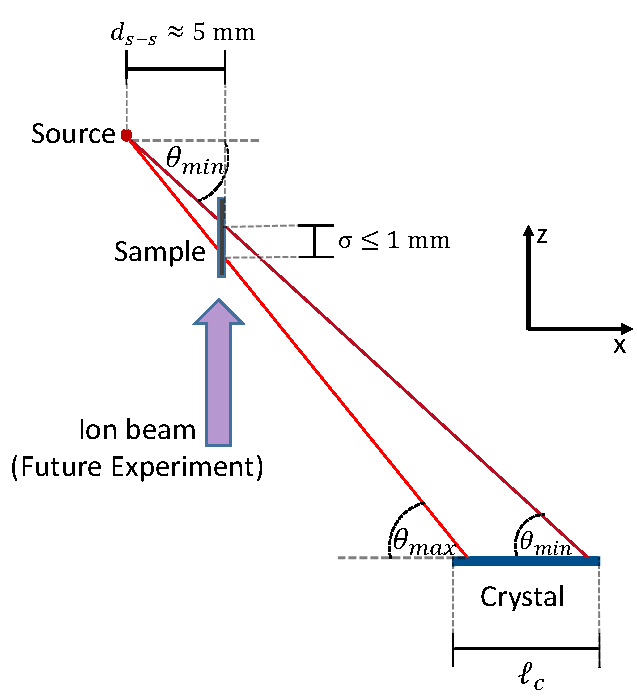
\includegraphics[width = 0.50\textwidth]{Diagrams/BraggAngleConstraint.pdf}
		\caption{Illustration of the sample size
			consideration. The length on the sample covered by x-rays in z direction 
			is denoted by 
			$\sigma$, which must stay at 
			or below \SI{1}{\milli\meter}. $\theta_{max}$ and 
			$\theta_{min}$ correspond to the 
			maximum and minimum Bragg angles of the 
			spectrometer respectively, while $\ell_c$ 
			represents the length of the crystal in the 
			dispersive plane and $d_{s-s}$ the source-sample 
			distance.}
		\label{BraggConstraint}
	\end{figure}
	\item \textbf{Spectral Resolution:} The main 
	requirement on the spectral resolution is 
	that it be high enough to resolve XAFS structures. From the example 
	spectrum given in fig. \ref{XAFS_examples}a, the required 
	resolutions can be estimated. Practically, 
	a spectral resolution of $\leq\SI{1}{\electronvolt}$ is expected to resolve the Al K-edge 
	sufficiently to carry out XANES, while $\sim$ 
	\SI{10}{\electronvolt} is required for EXAFS, estimated from 
	half of an oscillation period 
	\citep{levy2010double}. Spatial resolution 
	is 
	advantageous, but not a hard requirement. 
	\item \textbf{Intensity:} A high enough 
	intensity to resolve the spectra and perform 
	the absorption spectroscopy is necessary. In 
	the design this comes into play in part 
	through the length of the spectrometer and 
	distance to the source. Additionally the 
	choice of geometry and crystal play a role.
	\item \textbf{Physical Size:} The 
	spectrometers must fit in the HHT chamber. 
	This restricts the physical length to under 
	0.55 \unit{m}. There must also be space for the 
	heavy ion 
	beam in future experiments 
	and the PHELIX beam. 
\end{enumerate}


\section{Implemented Spectrometer Schemes}
\label{section: spectrometer geometries}
I designed two configurations according to the 
considerations above and the aspects discussed in the introduction to 
this chapter, namely a flat 
crystal geometry (see fig. \ref{BasicSpec}) 
and 
a bent crystal scheme, specifically a FSSR-1D geometry (see 
fig. \ref{FSSRSchemes}). For the flat crystal 
spectrometer, inspiration was 
drawn from \textit{Levy et. al.} \citep{levy2010double} and a dual channel 
geometry was chosen, so 
that both the transmitted and source spectrum can be 
simultaneously measured on a single detector. A flat crystal design has 
the advantage of simplicity in design and analysis of the spectra.

As for the bent crystal scheme, the 
FSSR-1D geometry offers the highest possible spectral 
resolution of FSSR schemes while also giving 
high luminosity on the detector. Additionally, it has the 
potential for 
1D imaging in the 
vertical direction, which could be exploited to 
simultaneously observe the 
source and transmitted spectra. I also considered a 
FSSR-2D configuration, but 
decided against it because some source spectra are 
expected to be smooth, 
which would significantly impact the spectral 
resolution. A von Hamos geometry was discarded because of its 
aforementioned shallow incidence angle on 
the detector, in contrast to the preferred quasi-perpendicular incidence on a CCD camera, and sensitivity to source 
broadening, 
which is altogether absent in the FSSR-1D scheme. 

The crystals for each scheme were chosen according to the considerations 
listed in the appendix, section \ref{section: crystal}, where the available crystal material choices and geometries influence each other so that a compromise must be found. In the end, I 
decided on using
ammonium dihydrogen phosphate (ADP) for the flat crystal geometry and 
mica for the bent crystal. ADP was 
chosen mainly for
its potential to reach 
extremely high optical and structural perfection as well 
as its lattice spacing of $2d_l = 
\SI{10.64}{\angstrom}$, allowing for diffraction in 
the first order, covering the 
desired energy range 
\citep{ferrari2019characterization, 
rajesh2015growth}. Mica was chosen for the FSSR-1D geometry for 
its bendability, high spectral 
resolution in tandem 
with good 
reflectivity, a wealth of previous applications in the 
literature and the possibility to use a low 
diffraction order (second order), yielding $2d_l/n = 
19.84/\SI{2}{\angstrom} = 
\SI{9.92}{\angstrom}$.
\citep{monot2002high,renner2019challenges,faenov1994,blasco2001portable}.
 One 
drawback of the mica crystal was that it contains 
aluminum, which could lead to 
a drop in reflectivity at the Al K-edge, though the 
expected decrease in 
intensity is not significant enough to exclude mica 
\citep{alkhimova2016determination}. Mica is also often 
used in FSSR 
spectrometers with strong bending, reaching radii of 
down to 
\SI{100}{\milli\meter} \citep{monot2002high}.

In addition to the two main spectrometers of this work, I will introduce 
another simple flat crystal spectrometer scheme in section \ref{section: SUCC}, which shares the geometry of a single channel of the flat crystal spectrometer I designed and
whose purpose is to deliver a wide energy range overview spectrum of the 
x-ray source as a control. It uses a potassium acid phthalate (KAP) 
crystal. This crystal is commonly used in x-ray spectrometers and has a 
larger rocking curve width than ADP \citep{kunze2009introduction, 
loisel2016measurement}. As this spectrometer is straightforward and not 
of my design, I will only describe it briefly and give its 
specifications.


\subsection{Dual Unbent Crystal Spectrometer}
\label{section:DUCC design}

\begin{figure} [H]
	\centering
	\begin{subfigure}[t]{0.48\textwidth}
		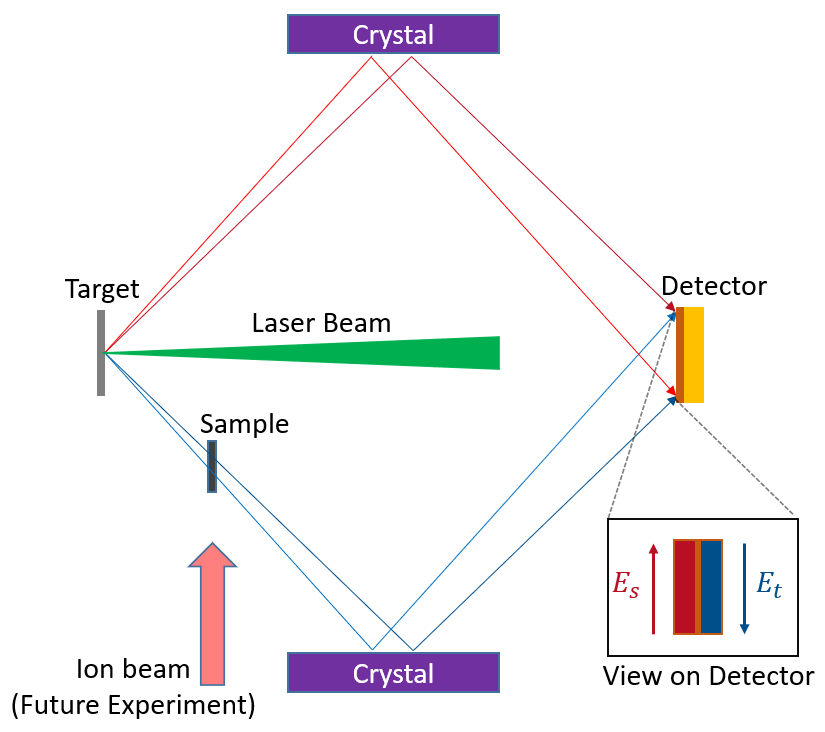
\includegraphics[width=\textwidth]{Diagrams/DUCCRealSchematic.PNG}
		\caption{Top view of the geometry, including a view on the detector which shows the detection of the source photons and transmitted photons with the energies $E_s$ and $E_t$, respectively.}
		\label{realDUCCSchematicTop}
	\end{subfigure}%
	\hfill
	\begin{subfigure}[t]{0.5\textwidth}
		\centering
		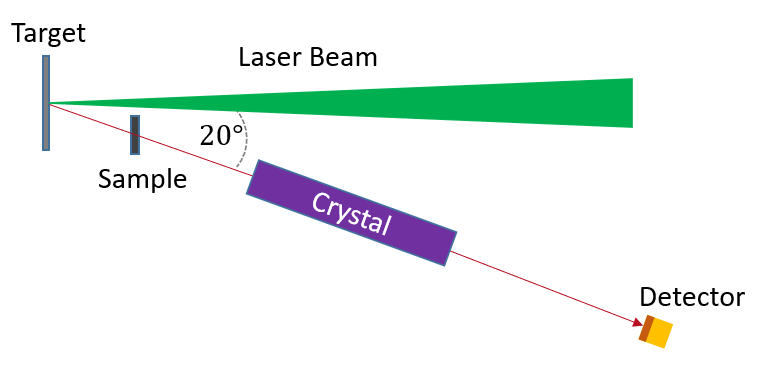
\includegraphics[width=\textwidth]{Diagrams/DUCCRealSchematicSide.PNG}
		\caption{Side view, in which the tilt of the 
			spectrometer is 
			illustrated.}
		\label{realDUCCSchematicSide}
	\end{subfigure}
	\caption{Schematic illustration of the DUCC geometry, not to 
		scale.}
	\label{realDUCCSchematic}
\end{figure}

The dual flat crystal spectrometer geometry, which I 
christened the \textbf{D}ual 
\textbf{U}nbent \textbf{C}rystal 
Spe\textbf{C}trometer (DUCC), is illustrated 
schematically in fig. \ref{realDUCCSchematic}. The 
central idea behind this 
geometry is to simultaneously record two spectra by 
implementing a mirror 
symmetrical two-channel design. This spatial symmetry 
ensures that the channels 
are illuminated by the same x-ray source, assuming a conical symmetry of the 
plasma emission. Through the combination of the DUCC geometry and ADP 
crystal, the DUCC spectrometer will target XANES and therefore 
have a relatively small energy range. This reduces the decrease of resolution due to source broadening and leverages the good crystal properties of the ADP.

In fig. \ref{realDUCCSchematicTop} the top view of 
the DUCC geometry is schematically shown. The laser beam 
irradiates the target, 
igniting a plasma. This plasma then emits soft x-rays, 
whose source spectrum is 
measured through the top channel using one half of the 
available detector 
surface. The transmitted 
spectrum through the sample, 
in this work an aluminum foil, is recorded through the 
bottom channel on the 
other half of the chip surface. The separation of the 
two spectra on the chip 
is realized by a plate with two openings inserted into 
the beam path before the 
two channels overlap (not shown in the figure). Space was 
left for the ion beam for 
future experiments, which 
is not a part of this work. To note is that 
space is left in the 
center of the spectrometer for a large lead block, which 
in the future will 
serve to shield the detector from protons being emitted from the sample due to the 
interaction with the heavy ion beam. Fig. 
\ref{realDUCCSchematicSide} depicts the $20\degree$ tilt 
of the DUCC spectrometer that I 
introduced to leave space for the laser beam, 
which is conical and has a half opening angle 
of $\pm 2.3\degree$. 
The 
spectrometer components 
were also tilted to simplify the design and deliver the 
simplest possible 
profile on the detector.




\subsection{Focusing Spectrograph with Spatial 
Resolution}

\begin{figure}[H]
	\centering
	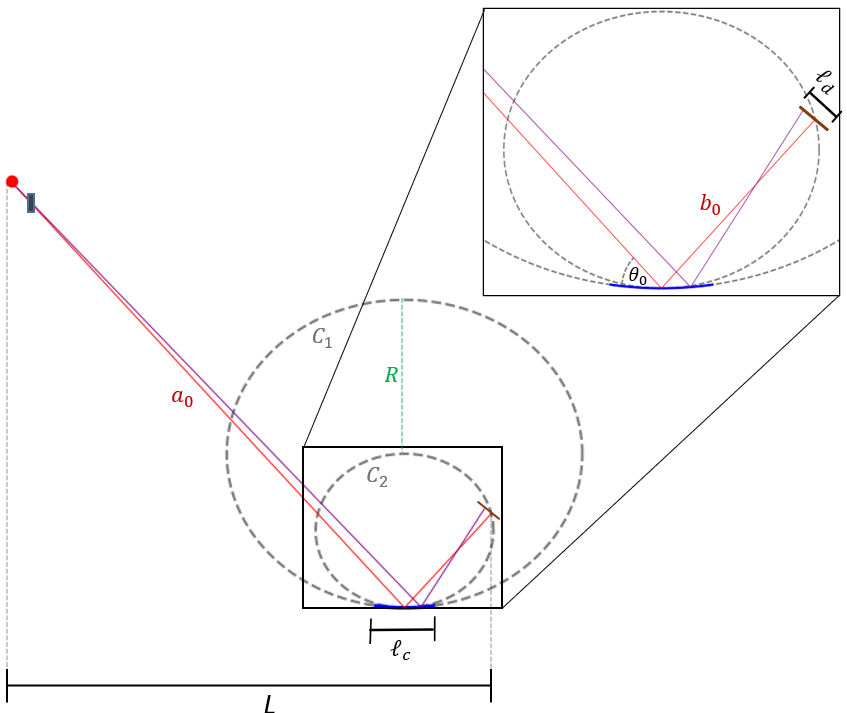
\includegraphics[width = 0.8\textwidth]{Diagrams/FSSRRealScheme.PNG}
	\caption{Schematic Illustration of the FSSR-1D, 
		where $R$ is the radius of curvature of the 
		crystal, $L$ the spectrometer length, $\ell_{c}$ 
		the length of the crystal in the dispersive plane 
		and $\ell_d$ the detector length in dispersive 
		direction. The crystal is depicted in blue, the 
		source in red and the sample in dark gray. Note 
		that the Rowland circle $C_1$ and circle drawn out by 
		the crystal curvature $C_2$ are also shown.}
	\label{realFSSRScheme}
\end{figure}

The FSSR-1D configuration used for the spectrometer with the curved crystal is 
depicted in fig. 
\ref{realFSSRScheme}. As the fundamental geometry 
effectively functions 
equivalently to the one 
described in section \ref{SectionTheoryFSSR}, I will 
not elaborate in detail on it here and instead discuss the spectrometer 
as a whole, 
so a FSSR-1D geometry with mica crystal. The main focus of this 
spectrometer is to capture a 
larger energy range, aiming to additionally resolve the oscillations in the 
EXAFS, 
while maintaining a good spectral resolution. 
Furthermore, the larger 
source-crystal distance $a_0$ and relation with the crystal-detector 
distance $b_0$ (see eq. \ref{Sfocusing}) allow freedom 
of placement in the chamber, as compared to the DUCC spectrometer. 
One 
potential drawback is 
the necessity of careful alignment and exact positioning 
of the components to 
achieve high spectral resolution, owing to the innate 
focusing and imaging of 
the FSSR scheme (see section \ref{SectionTheoryFSSR}). 

To note is that the potential of the 1D imaging for 
absorption spectroscopy with a single detector is not 
applied in this work due to the ratio of $a_0$ to $b_0$, 
leading to a magnification in the vertical plane of 
0.22. This magnification combined with the small 
sample size $\sigma$ renders an image too small to 
consistently differentiate between source and 
transmitted spectra. Despite this, the imaging 
properties find use in 
concentrating the x-rays from the plasma onto a 
single line in the dispersive direction on the 
detector, significantly reducing the effects of 
background, which will be especially advantageous in 
the future experiments with the heavy ion beam.

\subsection{Single Unbent Crystal Spectrometer}
\label{section: SUCC}
The \textbf{S}ingle 
\textbf{U}nbent \textbf{C}rystal 
Spe\textbf{C}trometer (SUCC) is a basic spectrometer, consisting of a 
single, flat crystal set in a geometry analogous to fig. \ref{BasicSpec} 
or to the top channel of the DUCC geometry (see fig. 
\ref{realDUCCSchematicTop}). Designed by P. Hesselbach, the spectrometer 
aims at a large enough energy range to cover both the FSSR-1D and DUCC 
spectrometer ranges, albeit at a lower resolution, owing to the source 
broadening intrinsic to the flat crystal geometry and the worse crystal 
properties of KAP as compared to ADP. To note is that the higher 
rocking curve width also increases the intensity on the detector, 
ensuring that control spectra are consistently recorded. Its role as a 
control implies that it will not be used for transmitted spectra.

In addition to the SUCC, another spectrometer by the name of old SUCC (OSUCC), a device used in a previous experiment and also designed by P. Hesselbach applying the same basic design as the SUCC, is used to extract spectra transmitted through a sample. The main purpose of the OSUCC in the experiment is to investigate the other aspects of the experimental setup by using an already tested spectrometer. In this work, it is used only when presenting qualitative results.

\section{Specifications and Comparison}
\label{section: specs and comparison}

For clarity and ease of discussion, I will for the rest of this work refer to the spectrometers by their geometries, i.e. DUCC, FSSR, SUCC, and OSUCC, where FSSR and FSSR-1D are interchangeable. If I specifically mean the geometries, I will append "geometry" onto the name, e.g. DUCC geometry.

Now that the specific geometries and crystal choices are 
established, I will introduce the specifications of each spectrometer 
and use them to 
validate that the considerations are fulfilled, 
as well as compare the spectrometers. The parameters are listed 
in table \ref{Table: Specs}. In the table, the first five parameters are 
directly 
relevant to the 
considerations presented in section \ref{section: design 
considerations}, where all but 
the spectral resolution follow directly from geometrical calculations. 
The spectral 
resolutions are derived using ray tracing simulations conducted with the python3 
code 
\textit{\textit{mmpxrt}} from Michal \v{S}m\'{i}d \citep{vsmid2021x}, the results of which are given in table \ref{TableResolutions}. For details 
on these 
simulations and path to the final resolution values, see section 
\ref{section: all 
simulations} in the appendix. In summary, the resolutions are calculated 
from three 
contributions: source broadening, detector resolution, and broadening 
from crystal 
properties. For the DUCC, the greatest contribution is due to source 
broadening, while 
for the FSSR-1D the crystal properties have by far the greatest impact. 
Additionally in the appendix, 
the dispersion for each spectrometer is determined from the simulations, 
and for the 
FSSR-1D with a simple ray-tracing code written by me, and compared to 
the analytical 
dispersions from section \ref{section:dispersion calculation}. For both 
spectrometers, 
the analytical and simulated dispersions show excellent agreement and 
are approximately 
linear, with the three different derivations for the FSSR-1D dispersion 
displaying near 
perfect overlap. 

\begin{table}[H]
	\centering
	\caption{Resolution contributions for the DUCC and FSSR-1D 
		spectrometers. 
		In both cases, the source broadening is taken from an 
		\textit{mmpxrt} simulation and assumes a source size of 
		\SI{150}{\micro\meter}, and the detector resolution 
		is calculated from the \textit{mmpxrt} dispersion and uses a 
		pixel size of \SI{13.5}{\micro\meter}. The 
		contribution due to the crystal properties for the 
		DUCC is estimated as described in section 
		\ref{section: DUCC Simulation}, while for the 
		FSSR-1D it is taken from \textit{mmpxrt}'s second $\Delta E$ 
		value. The total spectral resolution is calculated by using error propagation 
		on the source broadening and crystal properties' resolution, then linearly 
		adding on the detector resolution.}
	\vspace{0.05cm}
	\renewcommand{\arraystretch}{1.5}
	\centering
	\begin{tabular}{|c|c|c|} 
		\hline
		$\Delta E$ Contributions & DUCC 
		& FSSR-1D \\ [0.5ex]
		\hline\hline
		Source Broadening & \eV{0.621} & \eV{0.014} \\ 
		[0.5ex]
		\hline
		Detector & \eV{0.038} & \eV{0.143} \\ [0.5ex]
		\hline
		Crystal Properties & \eV{0.238} & \eV{2.954} \\ 
		[0.5ex]
		\hlineB{7}
		Total & \eV{0.703} & \eV{3.097} \\ [0.5ex]
		\hline
	\end{tabular}
	\label{TableResolutions}
\end{table}


The DUCC aims to resolve a narrow energy range around 
the 
Al K-edge to conduct XANES. Consequently, with a range of 1541-\SI{1618}{\electronvolt} this 
design successfully fulfills the energy range 
consideration. The sample size in z direction 
$\sigma$ is calculated using the geometry in fig. 
\ref{BraggConstraint}, as well as assuming a source 
size in z direction $s_z$ of \SI{150}{\micro\meter}, 
which yields the equation
\begin{equation}
	\sigma = (\tan\theta_{max} - 
	\tan\theta_{min})\cdot d_{s-s} + s_z,
	\label{eq: sample size DUCC}
\end{equation}
where $d_{s-s}$ corresponds to the source-sample 
distance of \SI{5}{\milli\meter} and $\theta_{max}$ and $\theta_{min}$ to the 
maximum and minimum Bragg angle of the 
spectrometer. This equation, along with the values in 
table \ref{Table: Specs}, result in a $\sigma$ of \SI{0.75}{\milli\meter}, so below the upper limit of \SI{1}{\milli\meter}, 
which together with the chosen $\theta_0$ and 
$d_{s-s}$ fulfill the sample size consideration. The 
spectral resolution of \SI{0.703}{\electronvolt} falls in the desired range of 
$\leq$\SI{1}{\electronvolt}. The small distances from source to detector 
address the intensity 
consideration, while a spectrometer length of \SI{235.17}{\milli\meter} easily complies with the 
physical size consideration of $\leq$\SI{550}{\milli\meter}. 

Next, the validity of the FSSR-1D will be 
assessed. With a 
maximum energy of 
\SI{1755}{\electronvolt}, the spectrometer is within 
the range to conduct EXAFS, fulfilling the energy 
range consideration. With a $\sigma$ of \SI{1.07}{\milli\meter}, the sample size is approximately equal to the upper limit of \SI{1}{\milli\meter},
where in this case the sample size is determined 
using the 3D-model of the FSSR-1D, 
as the angle of the sample w.r.t. the crystal depends on the 
placement of the FSSR-1D in the experimental setup described later in chapter \ref{chapter: experimental setup}. 
Accordingly, the sample size consideration is also 
achieved. With an energy resolution of 
\SI{3.097}{\electronvolt}, which is well under the 
requirement for EXAFS of \SI{10}{\electronvolt}, the 
spectrometer fulfills the spectral resolution 
consideration as well. The intensity 
consideration is addressed by the 
properties of the FSSR geometry. As with the DUCC, the FSSR-1D also 
fits well in the experimental chamber with a length of \SI{404.3}{\milli\meter}. Accordingly, all of the 
considerations outlined in the beginning of this 
chapter are fulfilled for both spectrometers.

I will now collect the arguments for each spectrometer interspersed 
throughout this chapter and present a comparison. Essentially for the 
purposes of this work, the question is whether to use a flat or bent 
crystal geometry, which depends also on the experimental conditions. The 
DUCC offers simplicity of design, easy alignment, and better crystal 
properties, at the cost of low collection efficiency and high 
sensitivity to source broadening. Conversely, the FSSR-1D boasts high 
collection efficiency, effective background reduction, and independence 
to source size, but is significantly more complex, difficult to align, 
and vulnerable to crystal defects caused by bending. As seen in table 
\ref{Table: Specs}, for both spectrometers the relative resolution, i.e. 
$\Delta E/(E_{max}-E_{min})$, is approximately the same at $\approx 1 
\%$. The sample size $\sigma$ and central Bragg angle $\theta_0$ are 
also comparable. This implies that neither spectrometer distinguishes 
itself solely in terms of its specifications, besides the fact that the DUCC is 
intended for XANES and the FSSR-1D for EXAFS. In conclusion, the more 
advantageous design will be determined largely qualitatively from its 
performance in the preparatory experiment, assuming that the derived 
numbers prove accurate.

Lastly, I will address the SUCC and its role in this work. As is apparent from table 
\ref{Table: Specs}, the SUCC covers a wider energy range than even the FSSR and 
therefore is intended for source characterization and acting as a control for the 
spectra of the DUCC and FSSR-1D. Another important aspect of this spectrometer is the 
chosen crystal, the KAP. This crystal material generally has a larger integrated 
reflectivity than the ADP ($\approx$80 and \SI{33}{\micro\radian} respectively 
\citep{gilfrich1975integral}), contributing to a 
higher intensity on detector. Consequently, a good signal to noise ratio is to be 
expected for most potential sources, further cementing its role as a control. Conversely, it is expected to display higher rocking curve widths than ADP, increasing the $\Delta E$ of the SUCC. Finally, 
this spectrometer design has been tested and vetted in previous experiments. As such, 
the SUCC can act as an effective backup, should either the DUCC or FSSR-1D have 
difficulties in the course of the experiment. 

\begin{table}[H]
\centering
\caption{Parameters of the DUCC with ADP crystals, FSSR-1D with mica 
crystal, and SUCC with KAP crystal. All 
spectrometers use a CCD camera as a detector. The parameters directly 
significant to the design considerations are listed 
first, followed by values that set the final geometry 
but are not immediately relevant to the 
considerations. The 
spectral resolution is 
calculated using the 
results from section \ref{section: simulation 
results}, summarized in table \ref{TableResolutions}. Source size is 
assumed to be \SI{150}{\micro\meter}.
Sample size $\sigma$ is
determined using eq. \ref{eq: sample size DUCC} for the DUCC and 
directly from the 3-D 
model for the FSSR-1D. In all cases, the source-sample distance is chosen to be \SI{5}{\milli\meter}.}
\vspace{0.05cm}
\renewcommand{\arraystretch}{1.5}
\centering
\begin{tabular}{|c|c|c|c|c|} 
\hline
Parameter & Denoted as & DUCC & FSSR-1D & SUCC \\ [0.5ex]
\hline\hline
Energy Range & - & 1541 - \SI{1618}{\electronvolt} & 1465 - 
\SI{1755}{\electronvolt} & 1400 - 
\SI{1800}{\electronvolt} \\ 
[0.5ex]
\hline
Bragg Angle Range & - & 46.01 - 49.14\degree & 45.4 - 58.53\degree & 
14.99 - 19.42\degree \\ 
[0.5ex]
\hline
Sample size (z) & $\sigma$ & 
\SI{0.75}{\milli\meter} & 
\SI{1.07}{\milli\meter} & 
- \\ [0.5ex]
\hline
Spectral Resolution & $\Delta E$ & 
\SI{0.703}{\electronvolt} & 
\SI{3.097}{\electronvolt} & - \\ [0.5ex]
\hline
Spectrometer Length & $L$ & \SI{235.17}{\milli\meter} & 
\SI{404.3}{\milli\meter}  & 
\SI{325.22}{\milli\meter} \\ [0.5ex]
\hlineB{7}
Central Bragg Angle & $\theta_0$ & 47.58$\degree$ & 51.36$\degree$ & 
17.23$\degree$ \\ 
[0.5ex]
\hline
Source-crystal Distance & $a_0$ & 
\SI{174.10}{\milli\meter} & 
\SI{549.71}{\milli\meter} & 
\SI{170.26}{\milli\meter} \\ [0.5ex]
\hline
Crystal-detector Distance & $b_0$ & 
\SI{174.10}{\milli\meter} & 
\SI{121.11}{\milli\meter} & 
\SI{170.26}{\milli\meter} \\ [0.5ex]
\hline
Detector Length & $\ell_d$ & \multicolumn{3}{|c|}{\SI{27.6}{\milli\meter}}
\\ [0.5ex]
\hline
Detector Width & - & \multicolumn{3}{|c|}{\SI{6.9}{\milli\meter}}
\\ [0.5ex]
\hline
Crystal Length & $\ell_c$ & 
\SI{40}{\milli\meter} & 
\SI{50}{\milli\meter} & 
\SI{50}{\milli\meter} \\ [0.5ex]
\hline
Crystal Width & - & 
\SI{30}{\milli\meter} & 
\SI{10}{\milli\meter} & 
\SI{20}{\milli\meter} \\ [0.5ex]
\hline
Crystal Radius & $R$ & - & 
\SI{155.04}{\milli\meter} & 
- \\ [0.5ex]
\hline
\end{tabular}
\label{Table: Specs}
\end{table}




